\section{Experimental results}
\label{sec: experiments}

% Bigger picture
There are many parameters involved in capturing the training images, extracting features, and training the random forest classifier. To study the contribution of these parameters, we systematically varied them and studied the accuracy of the resulting classifier. To study the accuracy, we set aside a collection of images as the test set and trained on a different set of images. We didn't use cross-validation due to the time constraints in training a random forest; it would have taken considerably longer time to test the cross validation accuracy and would  have prevented us from running as many tests as we did.

% Parameters tested
\subsection{Experiments}
We collected images of four different gestures shown in figure~\ref{fig:gestures}. We refer to each image that we captured as a ``training sample''. Since there are over 300000 pixels in each image, we sampled only 2000 of them so that we can train on more diverse images. From each image, we sampled 1000 background points, and 1000 points from the gesture to ensure we trained evenly on the different types of classes.

\textbf{Varying Parameters.} We varied three parameters in training the models. We varied the number of trees in the forest from two trees to five trees; 1000, 2000 and 3000 features; and different number of training images starting at 10, 50, 100 up to 350 increments of 50. We also set aside 50 images as the test set. For each of these 96 configurations, we trained a random forest model and computed the test set accuracy.

The features represent randomly selected offsets from the point of prediction. The offsets are radially sampled up to a maximum radius. We varied the radius of the sampling and generated feature files. We trained models with 2000 features, three trees, and different number of training images for radii set to 20, 40, 60, 100 and 200. \todo{WHAT UNIT IS THIS??? - mmpx. Explain this.}

Based on the results, we varied the parameters more in interesting directions: (1) We studied the effect of training a forest with just one tree, (2) we trained with 689 training images and 100 test images, and (3) we tried smaller radii for the feature offsets. 

In addition to varying the parameters, we conducted four more experiments. 

\textbf{Randomness.} First, due to the nature of the random forest, the trained model is non-deterministic and may yield a different accuracy rate for the same training set of images. In order to study this randomness, we trained ten models on the the same training set with 1000 features, 300 training images, and one tree. 

\textbf{SVM Comparison.} Second, we compared random forest classifier with a linear SVM classifier. We trained an SVM classifier for 2000 features, and different number of training images. 

\textbf{Pruning.} Third, we studied the effect of pruning on the accuracy of prediction. To study this, we pruned the forests trained with 2000 features and three trees for different number of training images. Then we calculated the test set accuracy of the pruned models.

\textbf{Overfitting.} Finally, we studied how much the model overfits to the training samples by calculating the training accuracy and comparing that with the test accuracy. We fixed 2000 features and three trees and varied the number of training samples. 

We used the ALGLIB \cite{alglib} for the random forest implementation, and LIBLINEAR \cite{liblinear} for SVM implementation.

\subsection{Results}

\begin{figure}
\begin{center}
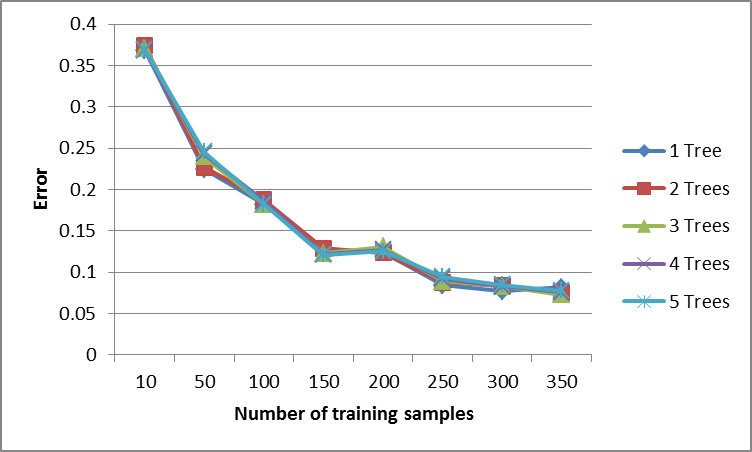
\includegraphics[width=0.45 \textwidth]{fig/varytrees.png}
\end{center}
\caption{We trained a classifiers with 2000 features, 350 training images and varied the number of trees from 1 to 8. The error is reported on a test set of 50 images.}
\label{fig:varytrees}
\end{figure}

\begin{figure}
\begin{center}
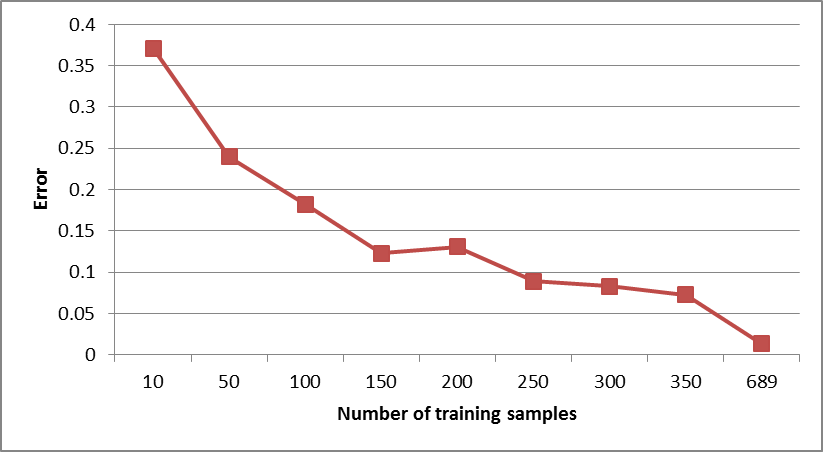
\includegraphics[width=0.45 \textwidth]{fig/largetraining.png}
\end{center}
\caption{We fixed the number of features at 2000, and the number of trees at 3 and varied the number of training images. Except for the last experiment, the error is reported on a test set of 50 images. Due to the size of the last training set, we increased the test set to 100 images.}
\label{fig:largetraining}
\end{figure}

\begin{figure}
\begin{center}
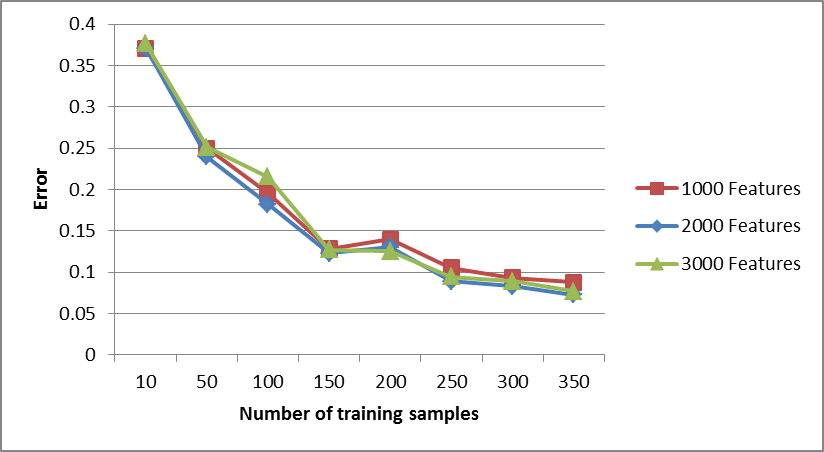
\includegraphics[width=0.45 \textwidth]{fig/varyfeatures.png}
\end{center}
\caption{We varied the number of features with three trees, and 350 training samples.}
\label{fig:varyfeatures}
\end{figure}


\begin{figure}
\begin{center}
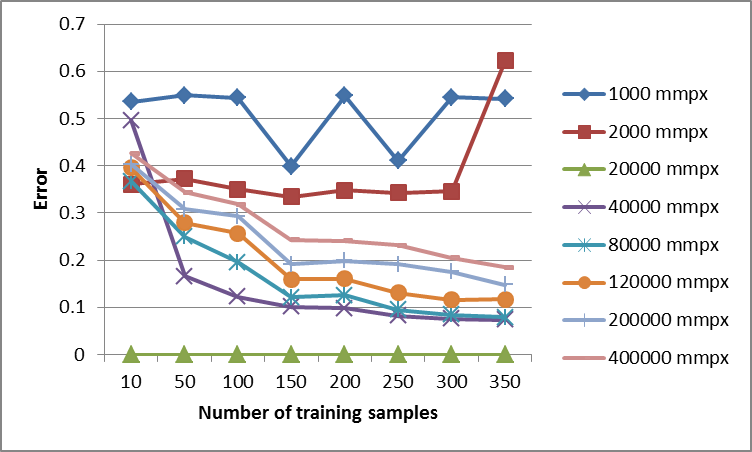
\includegraphics[width=0.45 \textwidth]{fig/varyradii.png}
\end{center}
\caption{We varied the maximum radius of the offsets used in generating the feature vectors. We fixed the number of features to 2000, and number of trees to 3.}
\label{fig:varyradii}
\end{figure}

\textbf{Varying Parameters.} Figure~\ref{fig:varytrees} shows the results of varying the number of trees while fixing the remaining parameters. We observed that the number of trees makes no noticeable difference. In fact, even training the forest with one tree has the same accuracy as the with multiple trees. This was also observed for different fixed values of the parameters. Adding multiple trees in the random forest is intended to protect against overfitting. However, our test and training sets were sampled from the same pool of images so we hypothesize one tree is sufficient to model all the variability in the test set. 

Figure~\ref{fig:largetraining} shows the effect of varying the number of training samples. There is a clear trend of smaller test error as we increase the number of training samples. At 689 training samples, the error is only 1.32\%. Increasing the number of training samples had the biggest impact in reducing the error when compared to other factors. 

Figure~\ref{fig:varyfeatures} shows the effect of varying the number features. Across most of our experiments we observed that using 2000 features outperforms 3000 features, which outperforms 1000 features. However, as seen in figure~\ref{fig:varyfeatures}, the difference in error is small. This suggests that if we sampled 1000, 2000, and 3000 features again, we may observe a different trend.

Finally, figure~\ref{fig:varyradii} shows the results of varying the radius of the offset features. For smaller training sample sizes, setting the radius to 40000 mmpx gives the least error classifier. However, as we increase the number of training samples, both 40000 mmpx and 80000 mmpx give similarly accurate classifiers. This means that when we have fewer training samples, setting the radius to 40000 mmpx will allow us to train a more accurate classifier, but when we have many training samples, the radius is not so important. We notice that making the radius too small or too large gives poor accuracy. By qualitatively checking the offset images as shown in figure~\ref{fig:offset}, we hypothesize that to train a more accurate classifier, the offsets should cover most of the hand, and then some of the background. If the radius is too small, then the offsets will be right next to each other and feature vectors for different gestures may be too similar.

\textbf{Randomness.} Training 10 models with the same parameters, we got a mean error of 9.82\% with 0.94\% standard deviation. The randomness is training the random forest is very concentrated around the mean. \todo{More? Or just leave this out?}


\begin{figure}
\begin{center}
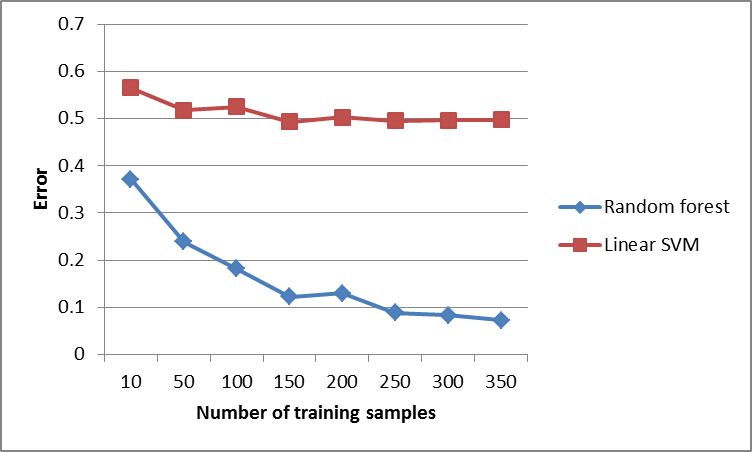
\includegraphics[width=0.45 \textwidth]{fig/linearsvm.png}
\end{center}
\caption{Using 2000 features, and 350 training images we trained a linear SVM and a random forest. The random forest was trained with 3 trees.}
\label{fig:linearsvm}
\end{figure}


\textbf{SVM Comparison.} Figure~\ref{fig:linearsvm} compares the error rate of a linear SVM with a random forest classifier. Linear SVM only slightly outperforms a random classifier that always predicts a pixel as the background. As we increase the training sample size, linear SVM improves much more slowly than the random forest.

\textbf{Pruning.} Pruning the tree showed almost no difference in accuracy compared to the full tree. We hypothesize the reason for this is that very high up in the tree the splitting nodes already confidently divide the training points into their class. However, ALGLIB continues to exhaust the features until the entire tree is constructed. By stopping the prediction early on in the tree, we don't suffer in accuracy, and improve the speed of prediction.

\begin{figure}
\begin{center}
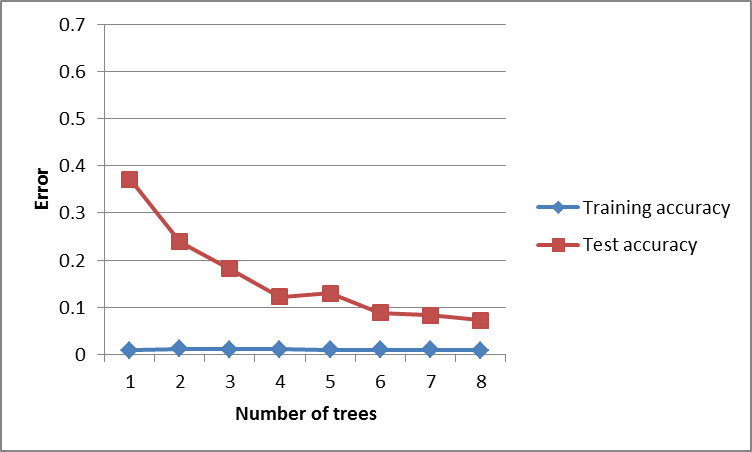
\includegraphics[width=0.45 \textwidth]{fig/trainingacc.png}
\end{center}
\caption{We fixed the number of features at 2000 and the number of trees at 3. For each training sample size, we compare the training accuracy and the test accuracy.}
\label{fig:trainingacc}
\end{figure}

\textbf{Overfitting.} Figure~\ref{fig:trainingacc} shows evidence of extreme overfitting. The training error is consistently very low (mean 1.06\%) and is much lower than the testing accuracy. 
